\acresetall
%%=========================================
\chapter{Discussion}\label{ch:Discussion}
In experiment~1, the evolution favoured agents that acted extrovert during the first generation, because most dialogues were unsuccessful and having many weak connections is better than having few weak connections. As the number of unique words decreased, dialogues became more likely to be successful, and a successful dialogue increases the involved agents' fitness. An extrovert agent had many edges, which increased its fitness. On the other hand, those edges had a lower average weight than an agent with fewer edges. A low average weight would decrease the agent's fitness. So there was a trade-off between acting introvertly and having fewer edges with high weights, and acting extrovertly and having more edges with lower weights. The population evolved towards favouring introvert characteristics. The new fitness function was designed so that both extrovert and introvert strategies have advantages and disadvantages. Considering that an extrovert strategy is optimal in the early stages and later on an introvert strategy is favourable, it seems that the fitness function gives room for both strategies to be viable. Which strategy is optimal depends on the environment and not the fitness function itself. 

Agents evolved towards higher learning rate, most likely because a high learning rate made the language easier to learn. When the population had almost reached consensus, and the average vocabulary size was close to $1.0$, the average learning rate stopped increasing. This might have happened because the pressure on being able to learn one language in a pool of many was gone. When only a few languages were being used, the pressure on having a high learning rate seems to drop. 

During first ten generations of experiment~1, the number of unique highest ranked words decreased. The agents that had edges of a certain weight survived the first generations. Those agents had a high fitness and were probable to be chosen as parents several times during the parent selection phase. The agents that got selected as parents several times and had a high probability of speaking to their children acquired more edges with strong weights, which increased their fitness and likelihood of surviving to the next generation. This cycle kept a select few agents alive for the first generations, allowing them to spread their language to many others. This is how the number of unique words dropped quickly during the first generations of the simulation. 

The average vocabulary size increased during the first seven generations of experiment~1, then it quickly decreased during the next three generations, and for the remainder of the simulation the average vocabulary length decreased slowly. During the first generations most agents did not have one word with a much higher weight than the others in the vocabulary, as seen in Figure \ref{fig:VocComp}. Because the words had similar weights, the probability of choosing the same word in each conversation was small, leading to words being spread around. In order to gain edges during the first generation, the agents favoured acting extrovertly. The combination of acting extrovertly and not choosing the same word in every conversation lead to the agents learning and teaching new words, which made the average vocabulary size increase. When a few words in the vocabularies had gotten a significantly higher weight than the others, those words were the only words that the newborn agents learned. The process where newborns only picked up the most successful words of their parents quickly reduced the number of unique words and the average vocabulary length. After the first ten generations, the evolution towards an average vocabulary length of 1.0 continued slowly because most words were highly weighted in someones' vocabulary.
 
The social network of experiment~1 became denser by each generation that passed up until generation $40$ which was when the average degree of the agents stabilised, as shown in Figure~\ref{fig:exp1.2}. Even though the agents mainly acted introvertly, the social network was not divided into groups, like in Lekvam’s experiment \citep[Section 5.1]{lekvam2014co}. The reason why this happened probably was because an agent could contact any other agent when it decided to act extrovertly. This meant that the entire population existed without any physical distance from one another. A community of individuals living so close to each other might have a social network similar to the one from this simulation. The network consisted of several circular layers, where the innermost layer had agents with the most edges, and the outer layer had the agents with the fewest edges.

Experiment~2 reached consensus after fewer generations than experiment~1, as seen in Figure~\ref{fig:hrwComp}. This happened because there were fewer words to begin with and fewer agents to teach one word to. An agent is more likely to become a parent in a small population, which leads to more newborns learning the same word from an earlier generation. The tendencies concerning how the language evolved were similar, only that it all happened faster with higher variance. In experiment~2 the average degree and fitness had especially big variations from one generation to another compared to experiment~1. See Figure \ref{fig:fitComp} for the fitness and Figure \ref{fig:degreeComp} for the degree. This is natural considering that there were randomness involved in the form of choosing the agents involved in dialogues, and making children. When fewer dialogues and fewer children were made per generation, the variance increase.

Experiment~3 should have less variance and require more generations to reach consensus than experiment~1 if this reasoning from experiment~2 was correct, and it did indeed have less variance and reached consensus later. The evolution began similarly to the two previous experiments, where the population's average degree, fitness and unique words evolved quickly. See Figure \ref{fig:fitComp} for the fitness, Figure \ref{fig:degreeComp} for the degree, and Figure \ref{fig:hrwComp} for the unique highest words. The population stabilised on a high number of unique words and a fitness of $0.5$. At generation $60$, the parents taught their children a few words and the average vocabulary size started decreasing, while the average fitness increased, see figure \ref{fig:VocComp}. This is exactly what happened in experiment~1, only that the population in experiment~3 required more time to reach a state where some words had a significantly higher weight than the rest of the words because of the population’s size. 

The social network of experiment~3 had small groups of two agents for many generations. Those small groups eventually died out or joined the main group because the agents in the small groups were unable to get a big enough fitness on their own. The evolution towards one social network happened more slowly than in the two previous experiments because the newborns in the main group learned many different words from their parents, giving the agents in the biggest group a lower average fitness than the biggest group in the two previous experiments.

The number of dialogues per generation was quintupled in experiment~4, and it would be natural to assume that it would allow the population to reach consensus faster than in the main experiment, but it did not, see figure \ref{fig:hrwComp}. It did, however, provide the agents with a higher average fitness because the average weight increased a lot due to the high number of introvert dialogues, see figure \ref{fig:fitComp}. The average degree decreased after the second generation because the parents taught their newborn agents fewer words than what they had in their own vocabularies, see figure \ref{fig:degreeComp}. However, the average quickly increased again, because the newborns shared their learned words through extrovert conversations. The number of extrovert conversations per agent per generation was naturally higher in this simulation. That lead to more newborn agents dying since their parents had a very high fitness, which the newborns could not compete with in the selection process. The parents' fitness was high because they had conducted so many dialogues during their lifetime that they had several highly weighted connections. This simulation required the same number of generations to reach consensus as experiment~1, which indicates that the number of dialogues had little effect on reaching consensus. This result leads to the conclusion that the dialogues had a small impact on the agents' vocabulary. The only other method for a newborn to learn a language in this model was through initial conversations with its parents, and experiment~4 indicates that parent-child dialogues might be important for the model to reach consensus.  

The fifth experiment tested the hypothesis that on the \textit{ontogenetic} time scale, which concerns how an individual learns language (\ref{EvoltionaryForces}), the most important factor is being taught a select few languages from an early age. In this model and in reality, the best method for being taught the same languages consistently is through several dialogues with the same persons, usually ones parents. This was tested through the probability of parents speaking to their newborn being set to three times less than in the main experiment. If the hypothesis was to be true, this experiment should have required more generations than the main experiment to reach consensus. Throughout the experiments performed thus far, when the average vocabulary length started decreasing, it seemed to be an indicator of that the population was approaching consensus. In experiment~1, the average vocabulary size started decreasing at generation eight, but in experiment~5, the average vocabulary size started decreasing at generation $25$, see figure \ref{fig:VocComp}. experiment~1 had reached consensus at generation $61$, while this experiment reached consensus at generation $127$, see figure \ref{fig:hrwComp}. This result supports the hypothesis that this computational model's most important factor for reaching consensus is the parents speaking to their children. This also indicates that the first dialogues are essential for the newborns' language in this computational model. The language of the children in the model is defined through their first dialogues, and after that it is very hard to change primary language, just like humans who tend to struggle when attempting to learn a language at an adult age. 

The average degree in experiment~5 was significantly lower than in experiment~1 because a lot of newborns did not get the initial dialogues with their parents, see figure \ref{fig:degreeComp}. The parent-child dialogues were reduced, but the experiment had the same number of dialogues, and therefore the same number of extrovert dialogues. This indicates that the average degree should be roughly $1/3$ of the main experiment. The main experiment stabilised on an average degree of about $10$, and this experiment stabilised on an average of about $4$, which is $2.5$ times as few edges as the main experiment.

The social network in experiment~5 evolved through a few agents that had a much higher fitness and a much higher probability of speaking to their children than the other agents in the population had. Those parents created the fan-like shapes, which were visible at generation $5$ and $10$. At generation $100$, the social network had evolved into a network similar to the network at generation $5$ from experiment~1. See Figure~\ref{fig:SNComparison} for snapshots of the social networks discussed. The network did not change during the last $50$ generations of the simulation. The fact that the social network in experiment~5 was much less dense indicates that the connections created through the initial dialogues were important when it comes to acquiring other connections than an agent's parents. This probably is because the probability of becoming a speaker is related to an agents' fitness. An agent without connections has a fitness of zero, making it unlikely that it would become a speaker. In experiment~5, many newborns did not have dialogues with their parents, which lead them to be unlikely to be chosen as speakers, which again lead to the social network being less dense compared to experiment~1.

\begin{figure}
    \centering
    \subfigure[]{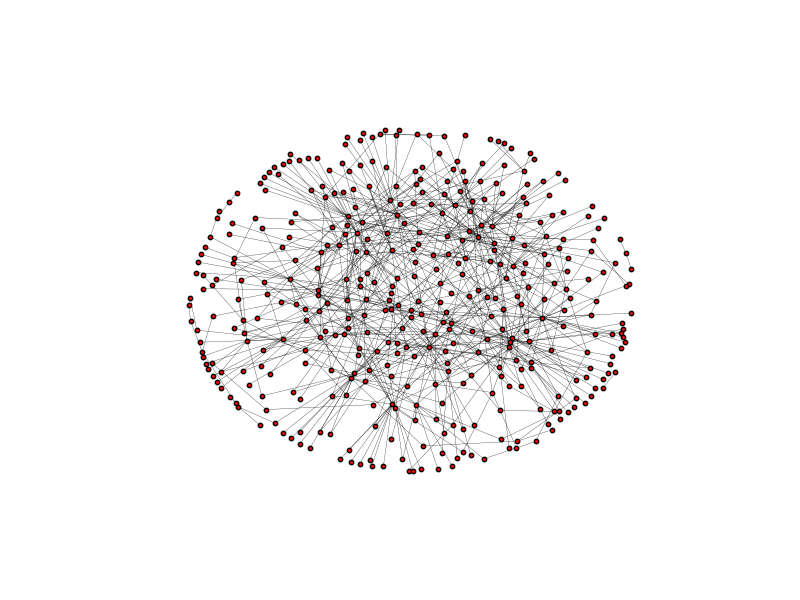
\includegraphics[width=0.32\linewidth]{fig/Results/Exp1/_graph5}\label{exp1SN5}}
    \hfill
    \subfigure[]{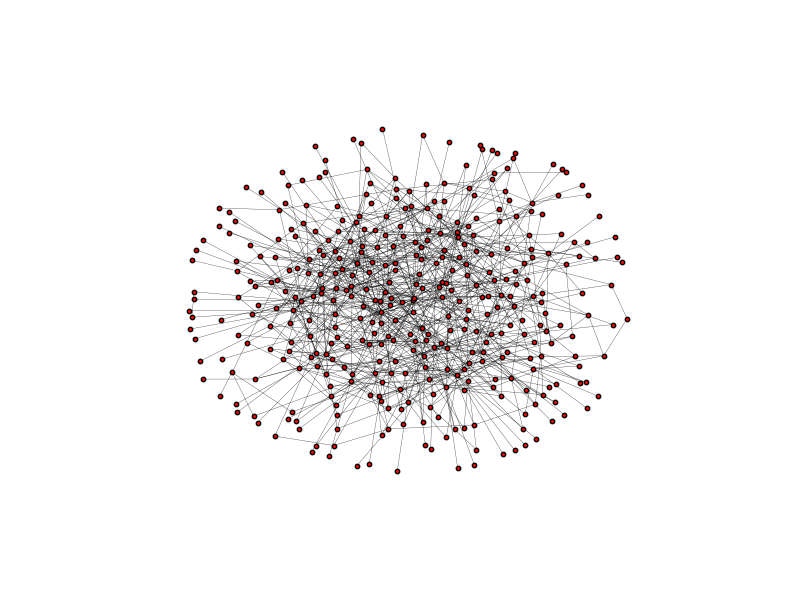
\includegraphics[width=0.32\linewidth]{fig/Results/Exp5/_graph100}\label{exp5SN100}}
    \hfill
    \subfigure[]{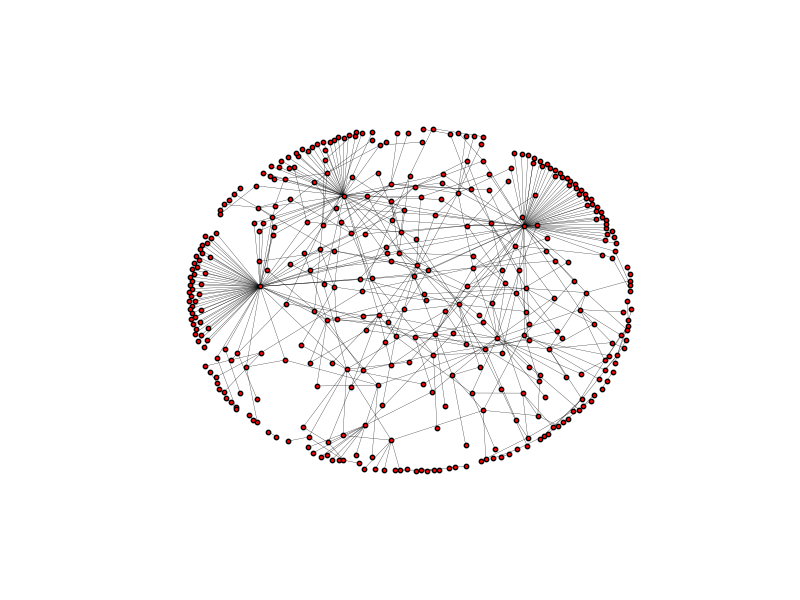
\includegraphics[width=0.32\linewidth]{fig/Results/Exp5/_graph5}\label{exp5SN10}}
    \hfill
    \caption{\subref{exp1SN5}: Experiment~1 at generation 5. \subref{exp5SN100}: Experiment~5 at generation 100. \subref{exp5SN10}: Experiment~5 at generation 10}
    \label{fig:SNComparison}
\end{figure}


If the number of newborns being produced per generation was less, one could expect to see similar results as the previous experiment, because with fewer newborns per generation, fewer newborns would conduct initial dialogues with their parents. Experiment~6 tested this through performing two experiments with increased $k$ and $n$ values. The results show that the population struggled to reach consensus; in fact, the population did not reach consensus within the $150$ generations ran in experiment 6a, see figure \ref{fig:hrwComp}. The result indicates that it is not only important to have many newborns being taught a consistent language in the early years, it is also important that a certain number of newborns are produced in each generation to allow the evolution to move forward. 

In experiment~6b an even larger portion of the population survived each generation, meaning that the selection pressure on the population was lessened even more. When the selection pressure was lessened, the evolutionary forces at the \textit{phylogenetic} and \textit{glossogenetic} time scale had less of an impact; see section \ref{EvoltionaryForces} for a description of the evolutionary forces. The small selection pressure in experiment~6b lead to the language evolving slower than in experiment~6a, see figure \ref{fig:hrwComp}. These results indicate that when the selection pressure on a species is small enough it does not need to evolve in order to survive, and then the species will evolve very slowly. In this computational model, when the selection pressure was high enough, the population reached consensus, but when the selection pressure was lessened the evolution towards consensus slowed down. This indicates that the Baldwin effect affects the \textit{phylogenetic} and \textit{glossogenetic} forces of language evolution. 

The average fitness and degree was higher when a larger part of the population survives to the next generation; see figure \ref{fig:fitComp} for the fitness and figure \ref{fig:degreeComp} for the degree. The agents who survive generally are among the fittest of the current population, and so when a larger portion of the agents with a high fitness survive, the average fitness becomes higher. The average degree is directly related to the fitness function, so it is natural that it is higher as well. \todo{legg til mer her}

In experiment~7a the agents could make up new words with a probability of $25\%$. One would expect that this made the percentage of successful dialogues to be less and the average vocabulary size to be bigger than in experiment~1. One might also expect that the population would have required more generations to reach consensus when a lot more utterances existed. As expected, the average fitness, degree, and percentage of successful dialogues in experiment~7a were lower than in experiment~1, and the average vocabulary size was a lot higher. See figure \ref{fig:VocComp} for the vocabulary, figure \ref{fig:fitComp} for the fitness, figure \ref{fig:degreeComp} for the degree and figure \ref{fig:DialogueComp} for the rate of successful dialogues. This did, however, not significantly affect the evolution towards consensus, as sees in Figure \ref{fig:hrwComp}. 

\begin{figure}
    \centering
    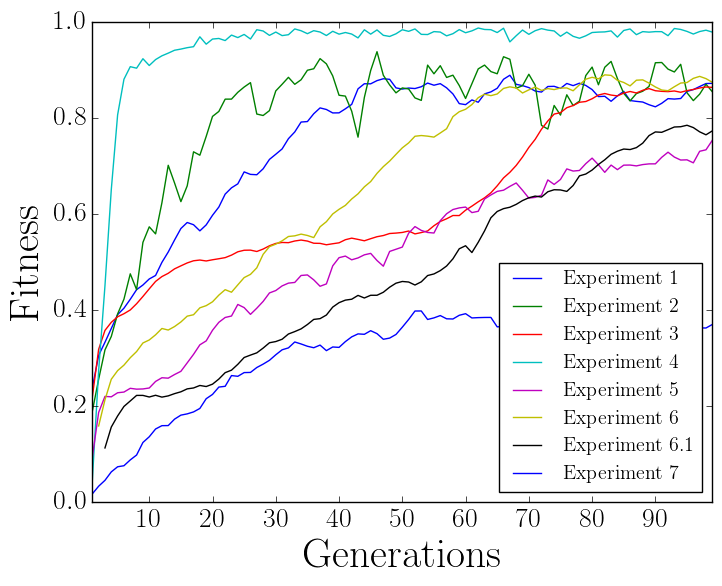
\includegraphics[width=0.7\linewidth]{fig/Discussion/FitnessComparison}
    \caption{Comparing the fitness per generation for experiment $1$, $2$, $3$, $4$, $6$, $6.1$, and $7.1$.}
    \label{fig:fitComp}
\end{figure}
\begin{figure}
    \centering
    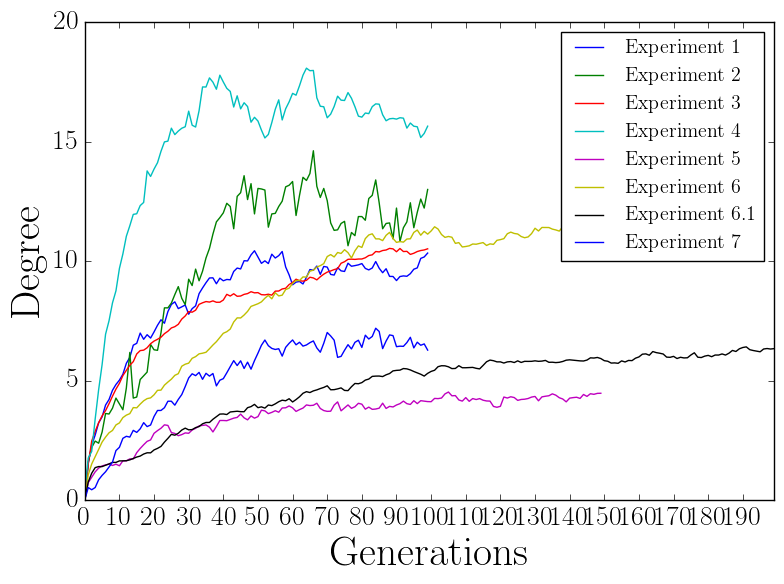
\includegraphics[width=0.7\linewidth]{fig/Discussion/DegreeComparison}
    \caption{Comparing the number of unique highest ranked words per generation for experiment $1$, $2$, $3$, $4$, $5$, $6$, $6.1$, and $7.1$.}
    \label{fig:degreeComp}
\end{figure}
\begin{figure}
    \centering
    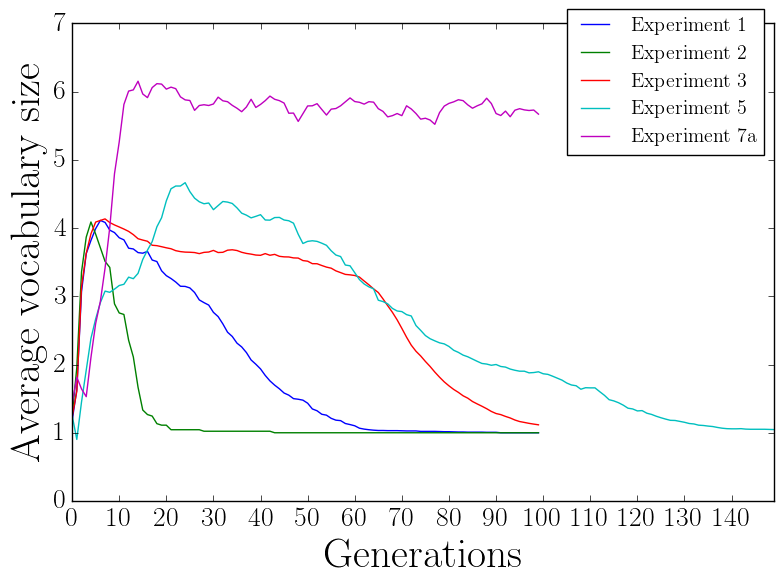
\includegraphics[width=0.7\linewidth]{fig/Discussion/VocabularyComparison}
    \caption{Comparing the average vocabulary size per generation for experiment $1$, $2$, $3$, $5$, and $7.1$.}
    \label{fig:VocComp}
\end{figure}
\begin{figure}
    \centering
    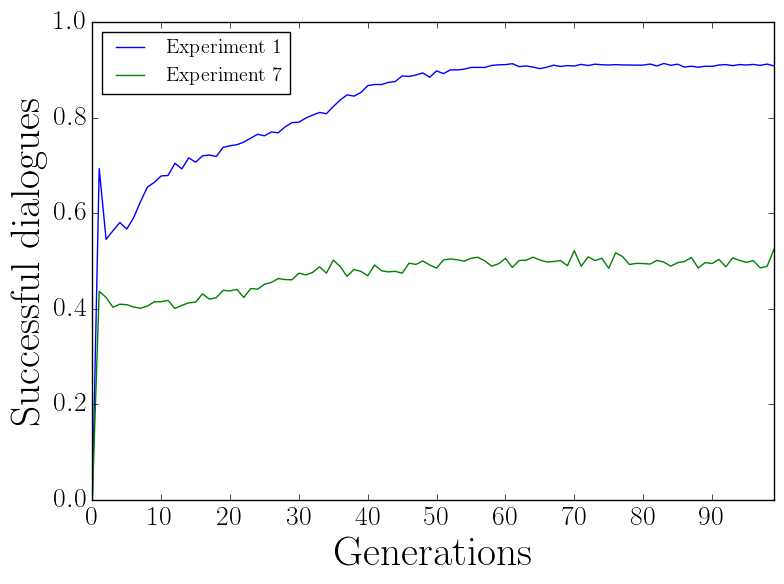
\includegraphics[width=0.7\linewidth]{fig/Discussion/DialogueComparison}
    \caption{Comparing the rate of successful dialogues per generation for experiment $1$ and $7.1$.}
    \label{fig:DialogueComp}
\end{figure}

The previous simulations that had struggled to reach consensus had forced the population to conduct less parent-child dialogues. This simulation actually did not force less parent-child dialogues. In fact, the probability of a parent choosing to utter a word from its vocabulary two out of the three dialogues it has with its newborn is $0.84$. The probability of at least one parent uttering at least two words from its vocabulary is $1 - (1-0.84)^2 = 0.97$. So the parent-child dialogues were not as affected by this as one might expect them to be. Also, the added number of words had very little impact, because they were weighted very low compared to the words that had survived for several generations. 

In experiment~7b the probability of inventing a word was increased to $45\%$, and the simulation struggled to reach consensus, as seen in Figure \ref{fig:hrwComp}. It seems that with a probability that high, several of the newborns were taught several words from their parents, leaving the newborns without consistent language to teach the next generation. When that happened to a large enough portion of the population, new words actually appeared in smaller groups for a few generations until the branch keeping the word alive died. The appearing and disappearing of these smaller languages happened regularly. After $73$ generations this simulation reached consensus. However, new words regularly appeared and disappeared, allowing the number of highest ranked words to vary between one and four from generation $73$ to generation $100$.

\begin{figure}
    \centering
    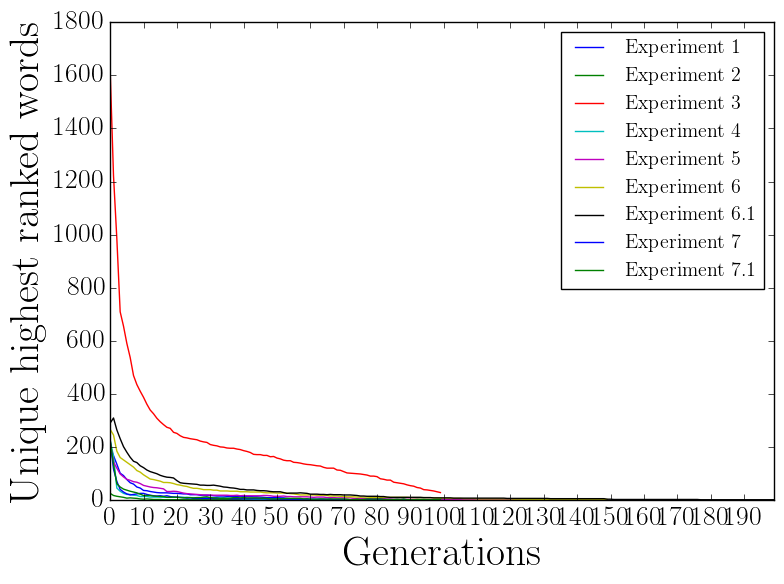
\includegraphics[width=0.7\linewidth]{fig/Discussion/hrwComparison}
    \caption{Comparing the number of unique highest ranked words per generation for experiment $1$, $2$, $3$, $4$, $5$, $6$, $6.1$, $7$, and $7.1$.}
    \label{fig:hrwComp}
\end{figure}